\section{Confidential Computing}
\label{sec:confidential-computing}

Moving on from the traditional distributed computing model, this section gives
an overview of the current state of confidential computing.

Data can be in three distinct states: ``at rest'', ``in transit'', and ``in
use''. These three states describe data stored in persistent storage, traversing
a network, and data currently being processed by an application. While
technologies protecting data at rest and in transit are commonly used today,
there are not many methods to protect data in use.

Confidential computing provides hardware-based primitives that allow the
creation of trusted execution environments (TEEs). These TEEs have specific
properties that protect data in use.

\subsection{Trusted Execution Environments (TEEs)}
\label{sec:tee}

\subsubsection{Properties}

There are different definitions of a trusted execution environment (TEE) with
varying properties. The three main properties defined by the
\textit{Confidential Computing Consortium} \cite{ccc2022technicalanalysis} are:

\begin{description}
  \item[Data confidentiality]
    Prevent unauthorized entities from viewing data that is in use within a TEE.
  \item[Data integrity]
    Prevent unauthorized entities from adding, removing, or changing data while
    it is in use within a TEE.
  \item[Code integrity]
    Prevent unauthorized entities from adding, removing, or changing code
    executed in the TEE.
\end{description}

Besides ensuring the confidentiality of data, code integrity is also critical
for the confidentiality of data. Even if data confidentiality is implemented
correctly, executing compromised code inside TEEs can also lead to confidential
data leakage.

Provided that the application code implements the computation correctly, data
and code integrity ensure that neither the data nor the application has been
modified, allowing clients to trust the results of the computations run inside
TEEs.

As TEE technologies widely differ in their implementations, this thesis will
treat the hardware and software components that create and protect TEEs as a
single platform consisting of all hardware and software components involved, and
refer to it as the ``TEE platform''.

Besides the three core properties, TEE platforms also often provide mechanisms
that enable the integration of a remote attestation process (see Section
\ref{sec:remote-attestation}), enabling clients to assess the trustworthiness of
TEEs created by an untrusted party. These technologies generally produce
evidence about the authenticity and integrity of both the TEE platform and
specific TEEs.

\subsubsection{Hardware Support}

The security of a software layer can only be as strong as the layers below it.
This is why an ideal security solution acts from the lowest layer possible. By
providing security through the lowest layer -- the hardware -- it is possible to
remove almost all software components between the hardware and the TEE from the
list of trusted components, including system software such as the operating
systems and hypervisors. The only components that need to be trusted are the
components of the TEE platform.

Today most TEE implementations still rely on firmware components that are part
of the TEE platform, allows manufacturers to deploy bug fixes and security
patches. Because an untrusted service provider can compromise these firmware
components, TEE platforms generally facilitate hardware-based mechanisms that
produce evidence about the integrity of the TEE platform.

\subsubsection{Memory Protection}

Most TEE technologies today rely on the protection of memory to provide the
three properties defined above. They often implement two mechanisms, protecting
the confidentiality and integrity of data stored in memory:

\begin{description}
  \item[Memory Encryption]
    TEE technologies rely on hardware components to encrypt data that is being
    transferred from the CPU to the physical memory of a machine and decrypt
    data moving from the memory to the CPU. Unlike homomorphic encryption, which
    provides specific computational functions directly on encrypted data
    \cite{monique2013homomorphicencryption}, TEE technologies transparently
    en-/decrypt data. Most importantly, the unencrypted data is only available
    while being processed by the CPU, and is encrypted before leaving the CPU.
    Memory encryption strengthens the confidentiality of data in use, as
    untrusted software components that gain access to the memory of a TEE or
    malicious entities that have physical access to the machine only see
    encrypted data.

  \item[Memory Access Control]
    On the other hand, memory integrity is guaranteed by enforcing that only the
    TEE owning a specific memory region can modify data stored in this region.
    In order to achieve this, the TEE platform has to keep track of protected
    memory pages, and their owners.
\end{description}

\subsection{TEE Models}
\label{sec:tee-models}

There are two distinct models of TEEs, process-based and VM-based.

\subsubsection{Process-based TEEs}
\label{sec:process-based-tees}

Process-based TEEs introduce a new programming model. A program needs to be
split into two components, trusted and untrusted. These are often referred to as
the ``enclave'' and ``host''. The enclave is executed in a TEE and, as such,
should contain all code that interacts with confidential data, whereas the host
component is responsible for handling non-sensitive tasks like networking and
file I/O.

While the host is not shielded, the enclave is protected from the rest of the
system, including:

\begin{itemize}
  \item the enclave's own host
  \item other processes running on the same machine
  \item the operating system
  \item firmware such as the BIOS
  \item the hypervisor and host operating system (in virtualized environments)
  \item hardware other than the processor
\end{itemize}

Splitting a program into enclave and host is challenging. It requires a deep
understanding of security and how these process-based TEE solutions work. SDKs
and frameworks often hide the split between host and enclave from developers to
ease the development of such applications \cite{schuster2022}.

Library OSes like Gramine and Occlum go even further and provide a POSIX-like
runtime environment with network, file I/O, and multithreading support. Because
applications running inside the enclave do not have access to the underlying OS,
library OSes provide libraries that implement OS system calls in the form of
library functions, while a boilerplate host provides I/O functionalities
\cite{tsai2014graphene}.

Even though these SDKs, frameworks, and library OSes ease the development, using
process-based TEEs still requires more development effort, and porting existing
applications often still requires the modification of the application.

\subsubsection{VM-based TEEs}
\label{sec:vm-based-tees}

The central concept of VM-based TEEs is to apply the TEE properties to a whole
virtual machine. Traditionally, hypervisors are fully responsible for managing
VM memory and thus have access to VM memory. On the other hand, TEE platforms
offering VM-based TEEs take away the responsibility of VM memory protection from
the hypervisor because the TEE platform itself already implements memory
protection. So instead of having full access to a VM's memory, the hypervisor
now only manages VM memory through mechanisms offered by the TEE platform.

VM-based TEEs are specifically designed to protect VMs from the rest of the
system, including:

\begin{itemize}
  \item VM firmware (e.g., OVMF)
  \item the hypervisor and/or host operating system
  \item hardware other than the processor
\end{itemize}

\subsubsection{Comparison}

Figure \ref{figure:cc-tee-comparison} compares the list of trusted components of
an application running without confidential computing, inside a process-based
TEE, and inside a VM-based TEE. In both TEE models the TEE platform enforces the
TEE properties and thus the hardware has to be partly trusted. 

On the one hand, process-based TEEs allow fine-grained separation of trust by
splitting applications into host and enclave, but this requires applications to
be ported to a new programming model. On the other hand, VM-based TEEs have much
larger attack surfaces because they include an entire OS but allow complex
applications to be run in a more secure environment without the need to modify
the applications.

\begin{figure}[H]
  \centering
  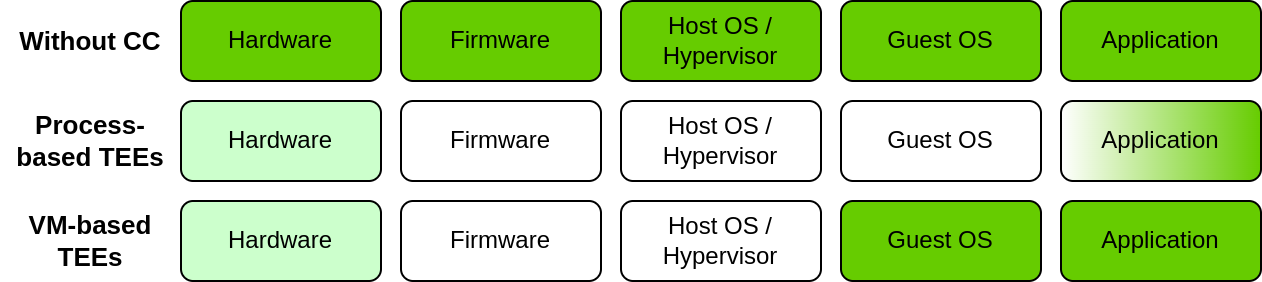
\includegraphics[width=0.85\linewidth]{resources/tee-models-comparison.drawio.png}
  \caption[Comparison of TEE models.]{
    Comparison of TEE models. In both TEE, cases the hardware has to be partly
    trusted, illustrated by the lightly marked hardware components. In the
    process-based TEE model, the application has to be split into enclave and
    host, which is why the application component is marked with a gradient.
  }
  \label{figure:cc-tee-comparison}
\end{figure}

\subsection{Commercially Available TEE Technologies}
\label{sec:commercial-tee-technologies}

\begin{description}
  \item[Intel SGX]
    Intel Software Guard Extensions (SGX) provides process-based TEEs by relying
    on hardware to create enclaves that contain application code and
    confidential data. As the name implies, it is an extension of Intel's CPU
    instruction set architecture \cite{costan2016sgx}.

    The CPU protects a designated memory area called the Processor Reserved
    Memory (PRM) established by SGX by ensuring that other software and hardware
    components, such as system software (hypervisor or OS) and DMA devices, do
    not have access to the PRM. Confidential data and enclave application code
    is stored in the Enclave Page Cache (EPC), a subset of the PRM. SGX relies
    on untrusted system software to manage EPC pages by assigning EPC pages to
    enclaves and evicting these pages if needed. However, system software cannot
    directly access the EPC, and the CPU maintains Enclave Page Cache Map (EPCM)
    in the EPC that keeps track of allocated EPC pages and the enclave which
    owns the page. Using the EPCM, the CPU checks the correctness of the system
    software's allocation decisions, ensures that an EPC page is only assigned
    to a single enclave, and that only the assigned enclave can access and
    modify the EPC page. The CPU also encrypts EPC pages while they are stored
    in physical memory to prevent leaking confidential data through PME attacks
    and guarantee the confidentiality of data stored in EPC pages after
    eviction.

    Initially, the system software asks the CPU to copy data from unprotected
    memory into EPC pages and assigns the pages to the enclave. After the EPC
    pages are loaded, the enclave is marked as initialized, and the system
    software can not access nor modify EPC pages anymore. The CPU then measures
    SGX firmware components and the EPC pages of the enclave, producing
    attestation evidence which is then signed by the CPU using a cryptographic
    key that is only accessible by the CPU. The signature can then be used to
    verify the authenticity of the evidence, which in turn can be used to verify
    the integrity of the enclave and the SGX platform. An attestation can not
    only be requested after initialization but also during runtime.

  \item[AMD SEV]
    AMD SEV-SNP is the latest iteration of AMD's Secure Encrypted Virtualization
    (SEV) technology \cite{amd2021sev, amd2017seves, amd2020sevsnp} and, as the
    name implies, provides VM-based TEEs.

    SEV relies on hardware-embedded encryption engines that encrypt or decrypt
    memory pages written to or read from the physical memory of a machine. It
    utilizes the AMD Secure Processor (AMD-SP), which is integrated into the
    same chip as the CPU, to generate and manage cryptographic keys used for the
    en-/decryption. All software and data are tagged with an Address Space
    Identifier (ASID). The CPU uses the ASID to restrict data access and
    modification to the owner with the same ASID, protecting data from any
    unauthorized usage. However, in the first iteration of SEV, the registers of
    a virtual CPU could be used to leak confidential data when shutting down a
    VM. Subsequently, AMD released their second iteration SEV-ES (Encrypted
    State), which encrypts VM memory and virtual CPU registers. The latest
    version SEV-SNP (Secure Nested Paging), introduced additional features that
    protect VM memory integrity.

    The attestation process for SEV VMs is similar to the attestation process
    for SGX enclaves. A hypervisor launches a VM, and after the VM is fully
    loaded, the VM's memory is encrypted. Subsequently, the AMD-SP measures SEV
    firmware components and VM memory pages, which are signed using a
    cryptographic key only accessible by the CPU. Again, the signature can then
    be used for verifying the authenticity of the measurements, and the
    measurements can be used for verifying the integrity of the VM and the SEV
    platform. Attestation support in SEV and SEV-ES was limited, as measurements
    could only be requested during the launch of a VM. SEV-SNP supports the
    request for measurements at any time, enabling a more flexible remote
    attestation.
\end{description}

\subsection{Limitations}
\label{sec:limitations}

\begin{description}
  \item[Performance Impact]
    Existing solutions require careful configuration to achieve acceptable
    performance or are inappropriate for specific use cases
    \cite{akram2021performance}. For example, due to the limited size of the EPC
    and the restricted programming model, Intel SGX displays a significant
    performance loss for high performance workloads, making the usage of SGX for
    these kinds of cases impractical.
  \item[CPU centric focus]
    Most of today's confidential computing solutions focus on a CPU-level view
    of memory permissions. This limits the application of confidential computing
    to heterogeneous computing systems, where discrete accelerators are used in
    order to speed up specific computations (e.g. GPUs and NPUs for machine
    learning workloads). However, there is ongoing work on integrating
    confidential computing into heterogeneous computing systems
    \cite{jiang2022cronus}.
  \item[New technology that requires further research]
    Since the introduction of Intel SGX in 2015, numerous vulnerabilities have
    been found in the SGX architecture \cite{fei2021sgxvulnerabilities}. AMD SEV
    has also not been spared, which until now required two iterations to fix the
    issues that have been discovered. Both technologies also depend on existing
    software, such as operating systems, hypervisors, and VM firmware, to
    implement the support of these technologies. These implementations also
    require further research and testing to find vulnerabilities and security
    issues.
\end{description}
